% =============================================================================
%  biomimetic_pipeline_schematic.tex -- end-to-end schematic, one page (letter).
%
%  Shows every stage of biomimetic-lattice-pipeline in order: upstream measurement
%  stack, ingest, the two JSON-schema contracts, the morphometrics-to-geometry
%  mapping, CAD + mesh, the target-stress FEA strain solver, metrics and pluggable
%  objectives, and orchestration including the closed-loop inversion.
%  Each stage names the package module that implements it.
%
%  Build (from docs/figures/src/):
%          pdflatex biomimetic_pipeline_schematic.tex
%          pdftoppm -png -r 200 -singlefile biomimetic_pipeline_schematic.pdf ../biomimetic_pipeline_detailed
%          cp biomimetic_pipeline_schematic.pdf ../../biomimetic_pipeline_schematic.pdf
%  Every acronym is expanded at first use.
% =============================================================================
\documentclass[10pt]{extarticle}

\usepackage[T1]{fontenc}
\usepackage[scaled=0.93]{helvet}
\renewcommand{\familydefault}{\sfdefault}
\usepackage{microtype}
\usepackage[letterpaper,margin=0.38in]{geometry}

\usepackage[dvipsnames]{xcolor}
\definecolor{hdrblue}{HTML}{00263A}
\definecolor{hdrteal}{HTML}{007A86}
\definecolor{hdrsky}{HTML}{4A9CB5}
\definecolor{slate}{HTML}{545B62}
\definecolor{biogreen}{HTML}{2E6B4F}   % biology / measured
\definecolor{mapmag}{HTML}{8E3B7E}     % the mapping layer
\definecolor{cadorange}{HTML}{B0620F}  % CAD / mesh
\definecolor{feared}{HTML}{8E3B46}     % FEA / metrics
\definecolor{objpurple}{HTML}{5B4B8A}  % objective / optimisation
\definecolor{gategold}{HTML}{B07D0F}
\definecolor{palebio}{HTML}{E9F2EC}
\definecolor{palemap}{HTML}{F6EDF4}
\definecolor{palecad}{HTML}{FBF1E4}
\definecolor{palefea}{HTML}{F8EBEC}
\definecolor{paleobj}{HTML}{EFEDF6}
\definecolor{paleblue}{HTML}{EAF2F5}

\usepackage[most]{tcolorbox}
\usepackage{tikz}
\usetikzlibrary{arrows.meta, positioning, calc, fit, backgrounds}
\usepackage{enumitem}
\usepackage{amsmath}

\setlength{\parindent}{0pt}
\pagestyle{empty}
\setlist[itemize]{leftmargin=10pt, itemsep=0.5pt, topsep=1.5pt, parsep=0pt}

\newcommand{\cmd}[1]{{\ttfamily\footnotesize\color{hdrblue}#1}}
\newcommand{\contract}[1]{{\ttfamily\footnotesize\bfseries\color{gategold}#1}}

\begin{document}

% =========================================================== PAGE 1 ==========
\begin{tcolorbox}[colback=hdrblue, colframe=hdrblue, boxrule=0pt, sharp corners,
                  left=8pt, right=8pt, top=5pt, bottom=5pt]
{\color{white}\Large\bfseries The biomimetic pipeline --- measured enamel $\rightarrow$ printable lattice}\\[2pt]
{\color{hdrsky}\footnotesize
\textbf{The problem it solves:} the measured morphometrics and the parametric lattice computer-aided-design (CAD) model existed \emph{separately} --- the CAD was driven by \textbf{hand-picked} parameters. \textbf{This pipeline makes the biology drive the geometry.}}
\end{tcolorbox}

\vspace{3pt}

\begin{center}
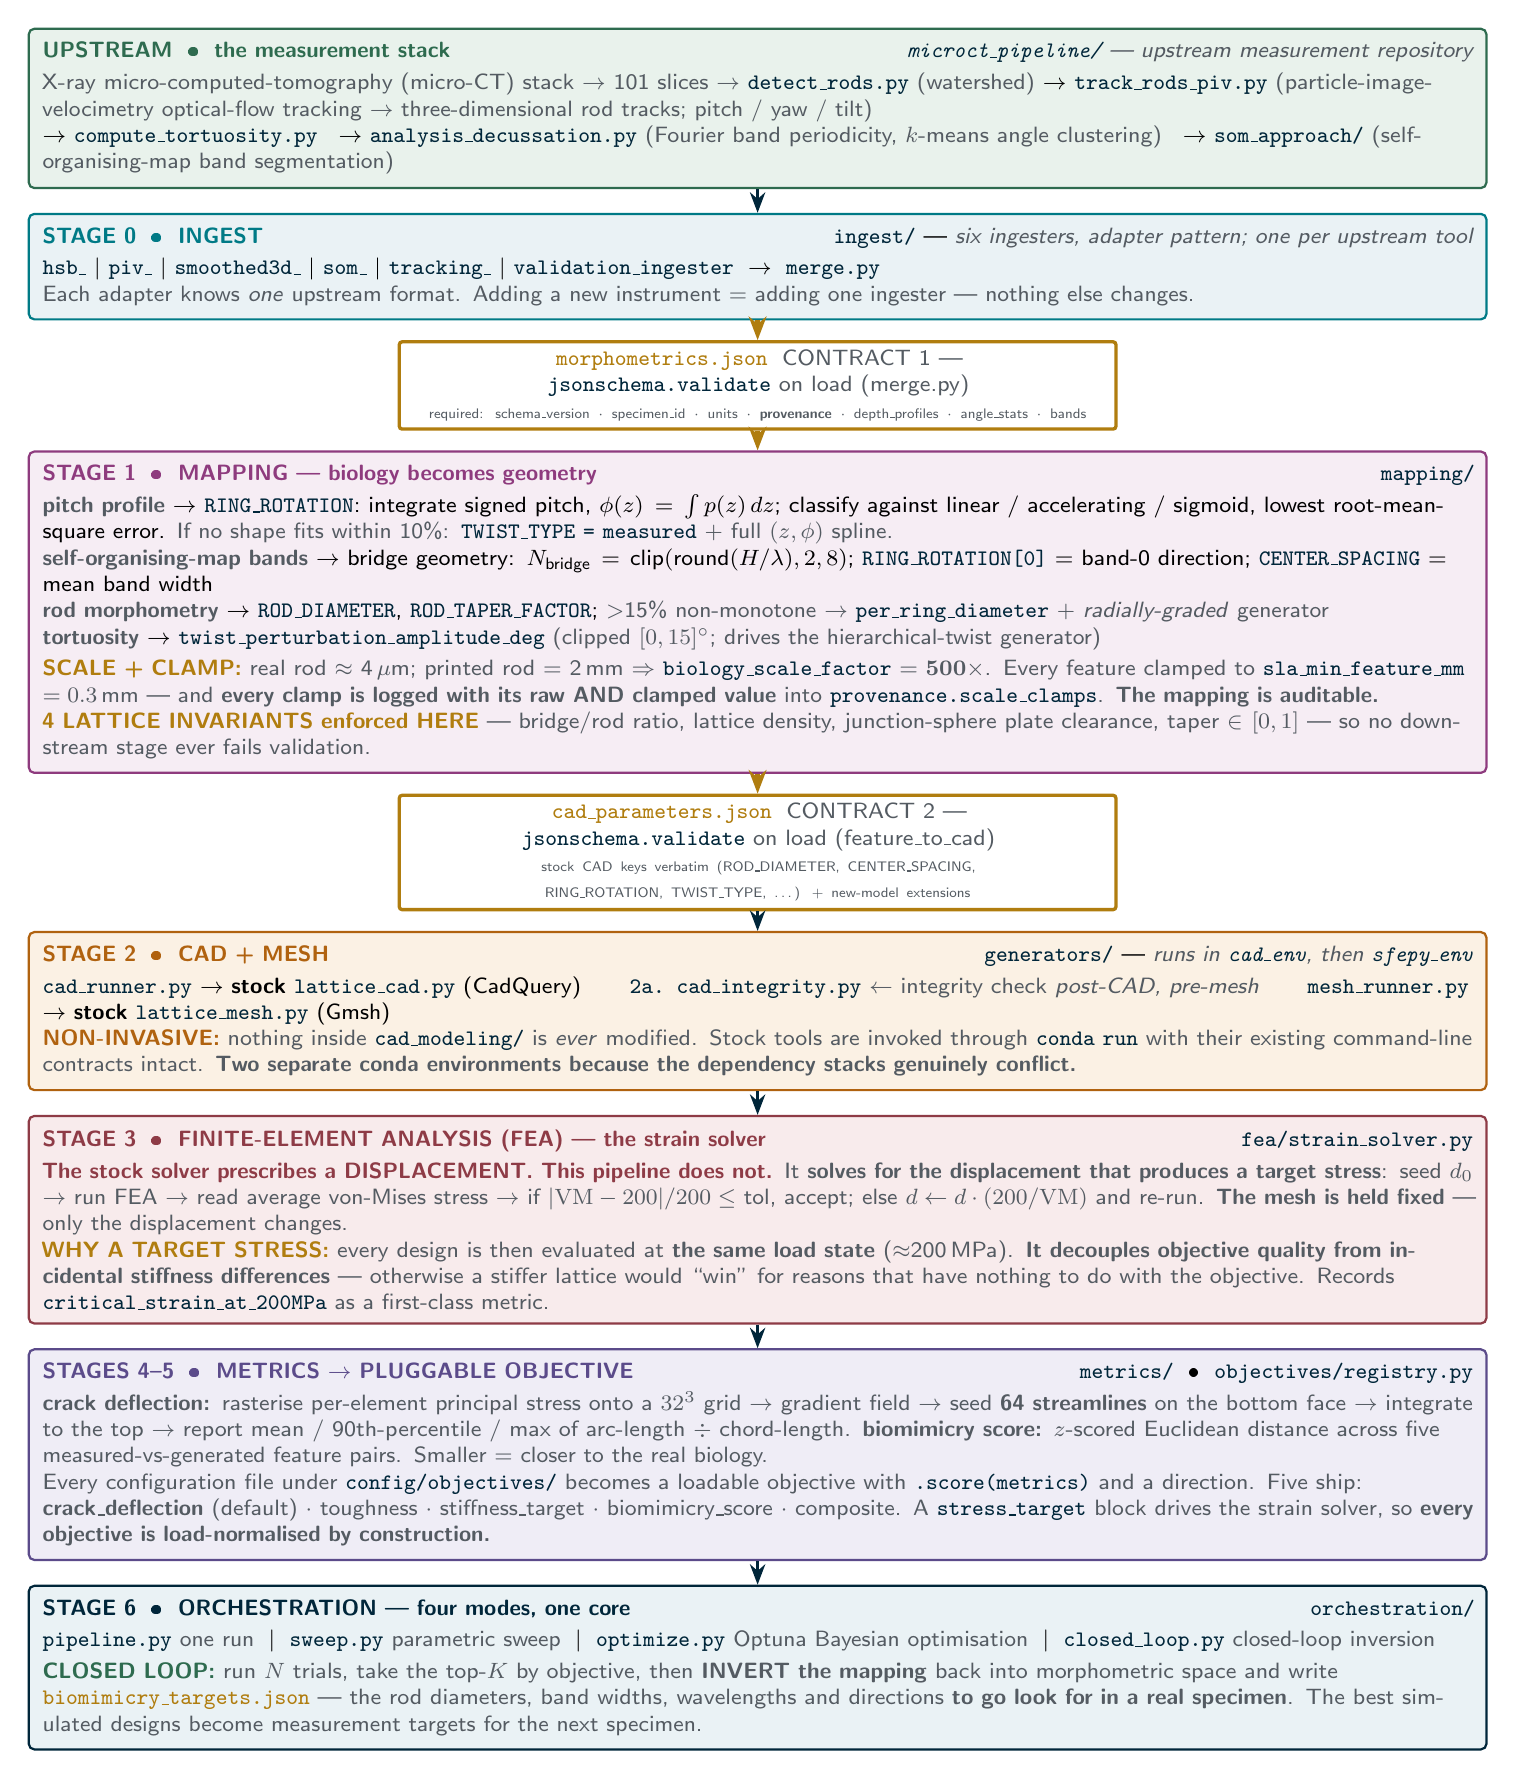
\begin{tikzpicture}[
  font=\footnotesize,
  stage/.style = {rectangle, rounded corners=2pt, draw=#1, line width=0.8pt,
                  align=left, inner sep=5pt, text width=7.15in},
  con/.style   = {rectangle, rounded corners=1pt, draw=gategold, line width=1.2pt,
                  fill=white, align=center, inner sep=3pt, text width=3.5in},
  flow/.style  = {-{Stealth[length=2.6mm]}, line width=1.0pt, draw=hdrblue},
  gate/.style  = {-{Stealth[length=3mm]}, line width=1.6pt, draw=gategold},
]

% ---- UPSTREAM (the research scripts) ----------------------------------------
\node[stage=biogreen, fill=palebio] (up) {
  {\color{biogreen}\bfseries UPSTREAM \;\textbullet\; the measurement stack} \hfill {\color{slate}\itshape \cmd{microct\_pipeline/} --- upstream measurement repository}\\[2pt]
  {\color{slate}X-ray micro-computed-tomography (micro-CT) stack $\rightarrow$ 101 slices $\rightarrow$}
  \cmd{detect\_rods.py} {\color{slate}(watershed)} $\rightarrow$
  \cmd{track\_rods\_piv.py} {\color{slate}(particle-image-velocimetry optical-flow tracking $\rightarrow$ three-dimensional rod tracks; pitch / yaw / tilt)}\\
  $\rightarrow$ \cmd{compute\_tortuosity.py} \;\;$\rightarrow$ \cmd{analysis\_decussation.py} {\color{slate}(Fourier band periodicity, $k$-means angle clustering)} \;\;$\rightarrow$ \cmd{som\_approach/} {\color{slate}(self-organising-map band segmentation)}
};

% ---- STAGE 0: INGEST --------------------------------------------------------
\node[stage=hdrteal, fill=paleblue, below=3mm of up] (ing) {
  {\color{hdrteal}\bfseries STAGE 0 \;\textbullet\; INGEST} \hfill \cmd{ingest/} --- {\color{slate}\itshape six ingesters, adapter pattern; one per upstream tool}\\[2pt]
  \cmd{hsb\_} \textbar\ \cmd{piv\_} \textbar\ \cmd{smoothed3d\_} \textbar\ \cmd{som\_} \textbar\ \cmd{tracking\_} \textbar\ \cmd{validation\_ingester} \;$\rightarrow$\; \cmd{merge.py}\\
  {\color{slate}Each adapter knows \emph{one} upstream format. Adding a new instrument = adding one ingester --- nothing else changes.}
};
\draw[flow] (up) -- (ing);

% ---- CONTRACT 1 -------------------------------------------------------------
\node[con, below=2.5mm of ing] (c1) {
  \contract{morphometrics.json} \;{\color{slate}CONTRACT 1 --- \cmd{jsonschema.validate} on load (merge.py)}\\
  {\color{slate}\tiny required: schema\_version $\cdot$ specimen\_id $\cdot$ units $\cdot$ \textbf{provenance} $\cdot$ depth\_profiles $\cdot$ angle\_stats $\cdot$ bands}
};
\draw[gate] (ing) -- (c1);

% ---- STAGE 1: MAPPING -------------------------------------------------------
\node[stage=mapmag, fill=palemap, below=2.5mm of c1] (map) {
  {\color{mapmag}\bfseries STAGE 1 \;\textbullet\; MAPPING --- biology becomes geometry} \hfill \cmd{mapping/}\\[2pt]
  {\color{slate}\bfseries pitch profile} $\rightarrow$ \cmd{RING\_ROTATION}: integrate signed pitch, $\phi(z)=\int p(z)\,dz$; classify against linear / accelerating / sigmoid, lowest root-mean-square error. {\color{slate}If no shape fits within 10\%: \cmd{TWIST\_TYPE = measured} + full $(z,\phi)$ spline.}\\
  {\color{slate}\bfseries self-organising-map bands} $\rightarrow$ bridge geometry: $N_{\text{bridge}}=\text{clip}(\text{round}(H/\lambda),2,8)$; \cmd{RING\_ROTATION[0]} = band-0 direction; \cmd{CENTER\_SPACING} = mean band width\\
  {\color{slate}\bfseries rod morphometry} $\rightarrow$ \cmd{ROD\_DIAMETER}, \cmd{ROD\_TAPER\_FACTOR}; {\color{slate}$>$15\% non-monotone $\rightarrow$ \cmd{per\_ring\_diameter} + \emph{radially-graded} generator}\\
  {\color{slate}\bfseries tortuosity} $\rightarrow$ \cmd{twist\_perturbation\_amplitude\_deg} {\color{slate}(clipped $[0,15]^\circ$; drives the hierarchical-twist generator)}\\[2pt]
  {\color{gategold}\bfseries SCALE + CLAMP:} {\color{slate}real rod $\approx$ 4\,$\mu$m; printed rod = 2\,mm $\Rightarrow$ \cmd{biology\_scale\_factor} $=\mathbf{500\times}$. Every feature clamped to \cmd{sla\_min\_feature\_mm} $=0.3$\,mm --- and \textbf{every clamp is logged with its raw AND clamped value} into \cmd{provenance.scale\_clamps}. \textbf{The mapping is auditable.}}\\
  {\color{gategold}\bfseries 4 LATTICE INVARIANTS enforced HERE} {\color{slate}--- bridge/rod ratio, lattice density, junction-sphere plate clearance, taper $\in[0,1]$ --- so no downstream stage ever fails validation.}
};
\draw[gate] (c1) -- (map);

% ---- CONTRACT 2 -------------------------------------------------------------
\node[con, below=2.5mm of map] (c2) {
  \contract{cad\_parameters.json} \;{\color{slate}CONTRACT 2 --- \cmd{jsonschema.validate} on load (feature\_to\_cad)}\\
  {\color{slate}\tiny stock CAD keys verbatim (ROD\_DIAMETER, CENTER\_SPACING, RING\_ROTATION, TWIST\_TYPE, \dots) + new-model extensions}
};
\draw[gate] (map) -- (c2);

% ---- STAGE 2: CAD + MESH ----------------------------------------------------
\node[stage=cadorange, fill=palecad, below=2.5mm of c2] (cad) {
  {\color{cadorange}\bfseries STAGE 2 \;\textbullet\; CAD + MESH} \hfill \cmd{generators/} --- {\color{slate}\itshape runs in \cmd{cad\_env}, then \cmd{sfepy\_env}}\\[2pt]
  \cmd{cad\_runner.py} $\rightarrow$ \textbf{stock} \cmd{lattice\_cad.py} (CadQuery) \;\;\;\;\;
  \cmd{2a. cad\_integrity.py} {\color{slate}$\leftarrow$ integrity check \emph{post-CAD, pre-mesh}} \;\;\;\;\;
  \cmd{mesh\_runner.py} $\rightarrow$ \textbf{stock} \cmd{lattice\_mesh.py} (Gmsh)\\
  {\color{cadorange}\bfseries NON-INVASIVE:} {\color{slate}nothing inside \cmd{cad\_modeling/} is \emph{ever} modified. Stock tools are invoked through \cmd{conda run} with their existing command-line contracts intact. \textbf{Two separate conda environments because the dependency stacks genuinely conflict.}}
};
\draw[flow] (c2) -- (cad);

% ---- STAGE 3: FEA -----------------------------------------------------------
\node[stage=feared, fill=palefea, below=3mm of cad] (fea) {
  {\color{feared}\bfseries STAGE 3 \;\textbullet\; FINITE-ELEMENT ANALYSIS (FEA) --- the strain solver} \hfill \cmd{fea/strain\_solver.py}\\[2pt]
  {\color{feared}\bfseries The stock solver prescribes a DISPLACEMENT. This pipeline does not.} {\color{slate}It \textbf{solves for the displacement that produces a target stress}: seed $d_0$ $\rightarrow$ run FEA $\rightarrow$ read average von-Mises stress $\rightarrow$ if $|{\rm VM}-200|/200 \le$ tol, accept; else $d \leftarrow d\cdot(200/{\rm VM})$ and re-run. \textbf{The mesh is held fixed} --- only the displacement changes.}\\
  {\color{gategold}\bfseries WHY A TARGET STRESS:} {\color{slate}every design is then evaluated at \textbf{the same load state} ($\approx$200\,MPa). \textbf{It decouples objective quality from incidental stiffness differences} --- otherwise a stiffer lattice would ``win'' for reasons that have nothing to do with the objective. Records \cmd{critical\_strain\_at\_200MPa} as a first-class metric.}
};
\draw[flow] (cad) -- (fea);

% ---- STAGE 4/5: METRICS + OBJECTIVE ----------------------------------------
\node[stage=objpurple, fill=paleobj, below=3mm of fea] (obj) {
  {\color{objpurple}\bfseries STAGES 4--5 \;\textbullet\; METRICS $\rightarrow$ PLUGGABLE OBJECTIVE} \hfill \cmd{metrics/} \;\textbullet\; \cmd{objectives/registry.py}\\[2pt]
  {\color{slate}\bfseries crack deflection:} {\color{slate}rasterise per-element principal stress onto a $32^3$ grid $\rightarrow$ gradient field $\rightarrow$ seed \textbf{64 streamlines} on the bottom face $\rightarrow$ integrate to the top $\rightarrow$ report mean / 90th-percentile / max of arc-length $\div$ chord-length.} {\color{slate}\bfseries biomimicry score:} {\color{slate}$z$-scored Euclidean distance across five measured-vs-generated feature pairs. Smaller = closer to the real biology.}\\
  {\color{slate}Every configuration file under \cmd{config/objectives/} becomes a loadable objective with \cmd{.score(metrics)} and a direction. Five ship: \textbf{crack\_deflection} (default) $\cdot$ toughness $\cdot$ stiffness\_target $\cdot$ biomimicry\_score $\cdot$ composite. A \cmd{stress\_target} block drives the strain solver, so \textbf{every objective is load-normalised by construction.}}
};
\draw[flow] (fea) -- (obj);

% ---- STAGE 6: ORCHESTRATION -------------------------------------------------
\node[stage=hdrblue, fill=paleblue, below=3mm of obj] (orch) {
  {\color{hdrblue}\bfseries STAGE 6 \;\textbullet\; ORCHESTRATION --- four modes, one core} \hfill \cmd{orchestration/}\\[2pt]
  \cmd{pipeline.py} {\color{slate}one run} \;\textbar\; \cmd{sweep.py} {\color{slate}parametric sweep} \;\textbar\; \cmd{optimize.py} {\color{slate}Optuna Bayesian optimisation} \;\textbar\; \cmd{closed\_loop.py} {\color{slate}closed-loop inversion}\\[2pt]
  {\color{biogreen}\bfseries CLOSED LOOP:} {\color{slate}run $N$ trials, take the top-$K$ by objective, then \textbf{INVERT the mapping} back into morphometric space and write} \contract{biomimicry\_targets.json} {\color{slate}--- the rod diameters, band widths, wavelengths and directions \textbf{to go look for in a real specimen}. The best simulated designs become measurement targets for the next specimen.}
};
\draw[flow] (obj) -- (orch);

\end{tikzpicture}
\end{center}

\end{document}
